\documentclass{article}
\usepackage[a4paper,top=3cm,bottom=2.5cm,left=2.5cm,
            right=2cm,marginparwidth=1.75cm,
            headheight=5pt]{geometry}
\usepackage[T5]{fontenc}
\usepackage[utf8]{inputenc}
\usepackage[document]{ragged2e}
\usepackage[vietnamese]{babel}
\usepackage[unicode]{hyperref}
\usepackage{amsmath}
\usepackage{setspace}
\usepackage{graphicx}
\usepackage{caption}
\usepackage{subcaption}
\usepackage{tcolorbox}
\usepackage{listings}
\usepackage{hyperref}
\usepackage{xcolor}
\usepackage{titlesec}
\usepackage{floatrow}
\usepackage[nottoc]{tocbibind}
\usepackage{mdframed}
\usepackage{amsmath}
\usepackage{amssymb}
\usepackage{tgbonum}
\usepackage{type1cm}
\usepackage{indentfirst}
\usepackage{lettrine}
\usepackage{colortbl}
\usepackage{fancyhdr}
\usepackage{wrapfig}
\usepackage{lastpage}
\usepackage{url}
\addto\captionsenglish{
  \renewcommand{\contentsname}{MỤC LỤC}%
  \renewcommand{\listfigurename}{Danh sách ảnh}%
  \renewcommand{\listtablename}{Danh sách bảng}%
  \renewcommand{\figurename}{Hình}
  \renewcommand{\tablename}{Bảng}
}
\pagestyle{fancy}
\fancyhf{}
\rhead{Toán ứng dụng và thống kê}
\lhead{\color{cyan}Đồ án 1: Color Compression}
\lfoot{Trang \thepage /\pageref{LastPage}}
\renewcommand{\footrulewidth}{0.4pt}
\setlength{\parindent}{5pt}
\setlength{\parskip}{1cm}
\renewcommand{\baselinestretch}{1.5}
\newmdenv[linecolor=black,skipabove=\topsep,skipbelow=\topsep,
leftmargin=2.5cm,rightmargin=2.5cm,
innerleftmargin=5cm,innerrightmargin=5cm]{mybox}
\usepackage{multicol}
\usepackage{indentfirst}
\usepackage{color}
\usepackage{apacite}
\usepackage{tikz}
\graphicspath{{Figures/}} 
\usepackage[square, numbers, comma, sort&compress]{natbib}  
\usepackage{lipsum}
\usetikzlibrary{calc}
\setlength{\columnseprule}{2pt}
\def\columnseprulecolor{\color{black}}
\def\maru#1{\textcircled{\scriptsize#1}}

\begin{document}
% Bìa trang
\begin{titlepage}
\begin{tikzpicture}[remember picture,overlay,inner sep=0,outer sep=0]
     \draw[blue!70!black,line width=4pt] ([xshift=-1.5cm,yshift=-2cm]current page.north east) coordinate (A)--([xshift=2cm,yshift=-2cm]current page.north west) coordinate(B)--([xshift=2cm,yshift=2cm]current page.south west) coordinate (C)--([xshift=-1.5cm,yshift=2cm]current page.south east) coordinate(D)--cycle;

     \draw ([yshift=0.5cm,xshift=-0.5cm]A)-- ([yshift=0.5cm,xshift=0.5cm]B)--
     ([yshift=-0.5cm,xshift=0.5cm]B) --([yshift=-0.5cm,xshift=-0.5cm]B)--([yshift=0.5cm,xshift=-0.5cm]C)--([yshift=0.5cm,xshift=0.5cm]C)--([yshift=-0.5cm,xshift=0.5cm]C)-- ([yshift=-0.5cm,xshift=-0.5cm]D)--([yshift=0.5cm,xshift=-0.5cm]D)--([yshift=0.5cm,xshift=0.5cm]D)--([yshift=-0.5cm,xshift=0.5cm]A)--([yshift=-0.5cm,xshift=-0.5cm]A)--([yshift=0.5cm,xshift=-0.5cm]A);


     \draw ([yshift=-0.3cm,xshift=0.3cm]A)-- ([yshift=-0.3cm,xshift=-0.3cm]B)--
     ([yshift=0.3cm,xshift=-0.3cm]B) --([yshift=0.3cm,xshift=0.3cm]B)--([yshift=-0.3cm,xshift=0.3cm]C)--([yshift=-0.3cm,xshift=-0.3cm]C)--([yshift=0.3cm,xshift=-0.3cm]C)-- ([yshift=0.3cm,xshift=0.3cm]D)--([yshift=-0.3cm,xshift=0.3cm]D)--([yshift=-0.3cm,xshift=-0.3cm]D)--([yshift=0.3cm,xshift=-0.3cm]A)--([yshift=0.3cm,xshift=0.3cm]A)--([yshift=-0.3cm,xshift=0.3cm]A);

   \end{tikzpicture}
\newcommand{\HRule}{\rule{\linewidth}{0.5mm}}
\center

\textsc{\Large TRƯỜNG ĐẠI HỌC KHOA HỌC TỰ NHIÊN}\\[0.5cm]
\textsc{\Large KHOA CÔNG NGHỆ THÔNG TIN}\\[1cm]

\includegraphics[width=0.3\textwidth]{logo/KHTN.jpg}\\[1cm]

\HRule \\[0.4cm]
{\huge \bfseries ĐỒ ÁN 1: COLOR COMPRESSION} \\[0.4cm]
{\large TOÁN ỨNG DỤNG VÀ THỐNG KÊ}\\[0.1cm]
\HRule \\[1.5cm]

\centerline{\Large{\textbf{Triệu Nhật Minh — 21127112 — 21CLC02}}}
\vspace{2.5cm}
\centerline{\large{\textit{Giảng viên hướng dẫn}}}
\vspace{0.25cm}
\centerline{\large{Vũ Quốc Hoàng}}
\centerline{\large{Lê Thanh Tùng}}
\centerline{\large{Nguyễn Văn Quang Huy}}
\centerline{\large{Phan Thị Phương Uyên}}

\vspace{2.5cm}
\centerline{\today}


\vfill % Wipe blank space of the page.
\end{titlepage}

% Mục lục tự động
\setlength{\parskip}{.5em}
\tableofcontents
\newpage

% Table of Figures & Tables
\setlength{\parskip}{.5em}
%\listoffigures
%\listoftables
\newpage

% Bắt đầu nội dung
\section{Hướng dẫn sử dụng}
\begin{description}
  \item[Bước 1:] Run all các cell trong notebook \textbf{21127112.ipynb} (hoặc chỉ run cell cuối cùng để chạy hàm main nếu đã khởi chạy các hàm bổ trợ từ trước).
  \item[Bước 2: ] Nhập đường dẫn tới ảnh cần nén (chỉ cần tên ảnh nếu ảnh đã nằm cùng thư mục với notebook).
  \item[Bước 3: ] Nhập số cụm màu cần nén (k\_cluster).
  \item[Bước 4: ] Nhập số lần lặp, số lần lặp càng cao thì ảnh được xử lý càng chính xác nhưng thời gian xử lý cũng càng lâu.
  \item[Bước 5: ] Nhập kiểu khởi tạo centroids (random hoặc in\_pixels).
  \item[Bước 6: ] Nhập định dạng lưu ảnh đầu ra (png hoặc pdf).
  \item[Bước 7: ] Ảnh đầu vào và ảnh sau xử lý được hiển thị song song để dễ dàng đối chiếu kết quả.
\end{description}

\section{Ý tưởng thực hiện}
\begin{description}
  \item[Bước 1: ] \label{view} Đọc ảnh đầu vào và chuyển về dạng mảng 1 chiều các điểm ảnh (img\_1d) nếu ta xem một điểm ảnh là một phần tử màu chứ không là bộ (tuple) các giá trị màu. Từ đoạn này trở về sau, ta sẽ giữ góc nhìn đối với mảng các điểm ảnh.
  \item[Bước 2: ] Chạy thuật toán K-Means. Trong thuật toán K-Means, ta cần khởi tạo các centroid ban đầu. Phụ thuộc vào cách khởi tạo centroids (random hoặc in\_pixels) mà ta sẽ có các cách khởi tạo khác nhau. Trong bài này, ta sử dụng 2 cách khởi tạo:
  \begin{itemize}
    \item \textbf{Random:} Chọn ngẫu nhiên k cặp giá trị màu, mỗi cặp giá trị gồm số kênh màu các giá trị trong khoảng từ 0 đến 255.
    \item \textbf{In\_pixels:} Chọn ngẫu nhiên k phần tử mảng 1 chiều img\_1d. Tuy nhiên, cách chọn ngẫu nhiên này sẽ không đảm bảo các centroid không bị trùng lặp. Do đó, ta cần tạo ra một mảng lưu các phần tử phân biệt (unique) của img\_1d. Sau đó, ta chọn ngẫu nhiên k phần tử trong mảng này.
  \end{itemize}
  Sau khi khởi tạo centroids, ta sẽ thực hiện các bước tiếp theo cho đến khi hết số lần lặp được yêu cầu. Một cách khác để dừng thuật toán là khi các centroid không thay đổi hoặc thay đổi rất ít so với lần lặp trước đó. Khái niệm ''rất ít'' ở đây được định nghĩa bằng một ngưỡng (threshold) được đưa ra trước. Trong đồ án này, ta sẽ cho threshold bằng 0, tức mảng centroids mới bằng mảng centroids cũ (liền trước) nó. Tại mỗi lần lặp, ta sẽ thực hiện 3 bước:
  \begin{itemize}
    \item Gán các điểm ảnh vào các cụm (clusters) tương ứng với centroids gần nhất.
    \item Tính toán lại vị trí các centroid mới bằng cách lấy trung bình cộng khoảng cách của tất cả các điểm ảnh trong cùng một cụm.
    \item Kiểm tra điều kiện dừng thuật toán.
  \end{itemize}
  \item[Bước 3: ] Sau khi thuật toán K-Means kết thúc, ta sẽ gán lại các điểm ảnh trong mảng img\_1d bằng các giá trị của centroids tương ứng.
  \item[Bước 4: ] Chuyển img\_1d về dạng mảng 2 chiều (img\_2d) và lưu ảnh đầu ra theo định dạng đã cung cấp (png hoặc pdf).
\end{description}

\section{Mô tả}
% Template mô tả hàm
% \textbf{Input:} \\
% \textbf{Output:}

% \paragraph{Mô tả:}
\subsection{Nhóm hàm chính}
\subsubsection{get\_labels}
\textbf{Input:} Mảng 1 chiều các điểm ảnh, mảng các centroid \\
\textbf{Output:} Mảng các nhãn của các điểm ảnh, phần tử thứ i của mảng này là nhãn của điểm ảnh thứ i trong mảng điểm ảnh đầu vào, giá trị của phần tử này nằm trong khoảng $[0, k - 1]$ ($k$ là số cụm)

\paragraph{Mô tả:}
Mục đích của hàm là áp dụng công thức khoảng cách Euclid để xác định khoảng cách
giữa mỗi điểm ảnh và các centroid. Tiếp theo, ta sẽ gán nhãn của centroid gần nhất cho điểm ảnh
đó. Để tính toán khoảng cách, ta sử dụng hàm numpy.sum với tham số \textit{axis=-1} để thực hiện phép cộng theo chiều cuối cùng của mảng, tức là chiều kênh màu. Để có thể tính được khoảng cách, ta cần reshape lại mảng điểm ảnh và mảng centroid để có thể áp dụng broadcasting. 

\paragraph*{Broadcasting}
là kỹ thuật cho phép numpy thực hiện các phép toán trên các mảng có kích thước khác nhau mà không cần phải lồng các vòng lặp. 

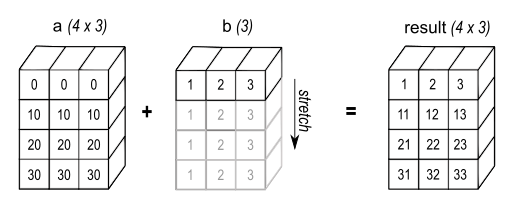
\includegraphics[width=0.5\textwidth]{image/broadcasting_2.png}

Trong trường hợp này, ta sẽ reshape mảng điểm ảnh về kích thước (số điểm ảnh, 1, số kênh màu) và mảng centroid về kích thước (1, số cụm, số kênh màu). Sở dĩ cần reshape vì điều kiện để broadcasting là các chiều của 2 mảng phải bằng nhau hoặc bằng 1. Khi này, mảng centroids sẽ thực hiện nhân bản để thực hiện phép trừ với mỗi điểm ảnh.

Sau đó, ta sẽ sử dụng hàm numpy.sum để tính tổng bình phương khoảng cách giữa mỗi điểm ảnh và các centroid. Hàm numpy.argmin sẽ trả về chỉ số của centroid có khoảng cách nhỏ nhất với điểm ảnh đó. Cách ép kiểu dữ liệu của mảng điểm ảnh và mảng centroid về kiểu int64 trước khi tính toán là để tránh tràn số khi tính toán (ví dụ: $1 - 255 = 1$ thay vì $-254$ nếu ta giữ nguyên kiểu dữ liệu uint8). Việc ép kiểu này không ảnh hưởng đến giá trị của mảng labels trả về vì thực chất ta chỉ cần biết chỉ số của centroid gần với điểm ảnh nhất.

\subsubsection{initialize\_centroids}
\textbf{Input:} Mảng 1 chiều các điểm ảnh (img\_1d), số cụm (k\_cluster) và kiểu khởi tạo (init\_centroids) \\
\textbf{Output:} Mảng các centroid

\paragraph*{Mô tả:} Đầu tiên, ta cần đếm số màu phân biệt trong bức ảnh (sử dụng numpy.unique) và so sánh chúng với số màu cần ''nén''. Sử dụng hàm min để lấy giá trị nhỏ nhất giữa 2 giá trị để đảm bảo số màu cần ''nén'' không vượt quá số màu phân biệt trong bức ảnh. Sau đó, tuỳ thuộc vào kiểu khởi tạo centroids người dùng nhập vào (random hoặc in\_pixels) thì hàm sẽ khởi tạo các centroid theo kiểu tương ứng:
\begin{description}
  \item [random:] Sử dụng numpy.random.randint để tạo ra một mảng các số nguyên ngẫu nhiên trong khoảng từ 0 đến 255 với số sample trả về bằng số cụm, mỗi cụm có số kênh màu giá trị (ở đây số kênh màu là img\_1d.shape[1] do số kênh màu trong đa số các trường hợp test là 3 (tương ứng với hệ màu RGB), tuy nhiên có trường hợp số kênh màu trả về là 4. Do đó để đảm bảo tính tổng quát, ta sẽ sử dụng img\_1d.shape[1]), đồng thời ép kiểu giá trị trả về là số nguyên không âm 8bit để đảm bảo tính chính xác của giá trị trả về.
  \item [in\_pixels:] Sử dụng numpy.random.choice đồng thời tận dụng mảng unique\_img\_1d lưu trữ các màu phân biệt trong bức ảnh để tạo ra mảng các màu ngẫu nhiên với số kết quả trả về là số cụm. Sau đó lấy ra phần tử tương ứng trong mảng unique\_img\_1d và gán chúng làm giá trị cho phần tử trong mảng centroids. Mỗi cụm có số kênh màu bằng với số kênh màu của phần tử trong mảng unique\_img\_1d. Trong lúc random xuất hiện một tham số \textit{replace=False} nhằm đảm bảo các màu được chọn không có sự trùng lặp.
\end{description}
Nếu giá trị của tham số init\_centroids không phải là ''random'' hoặc ''in\_pixels'' thì hàm sẽ báo lỗi. Và dù bằng bất kì cách random hợp lệ nào thì mảng centroid trả về đều được chuyển thành ndarray 2 chiều với số hàng (rows) bằng số cụm, số cột (cols) bằng số kênh màu của phần tử trong mảng img\_1d (img\_1d.shape[1]).

\subsubsection{update\_centroids}
\textbf{Input:} Mảng 1 chiều các điểm ảnh (img\_1d), mảng các nhãn (labels), số cụm (k\_clusters) và mảng các centroid (centroids) \\
\textbf{Output:} Mảng các centroid mới được cập nhật (new\_centroids)

\paragraph{Mô tả:}
Với nhiệm vụ cập nhật lại các tâm cụm dựa trên dữ liệu ảnh một chiều và nhãn của từng điểm ảnh, hàm có 4 đối số đầu vào là img\_1d, labels, k\_clusters và centroids. Biểu thức \textit{np.mean(img\_1d[labels == i], axis=0)} sẽ trả về giá trị trung bình của các điểm ảnh có nhãn i trong mảng img\_1d. \textit{if img\_1d[labels == i].size > 0} sẽ kiểm tra xem có phần tử nào trong mảng img\_1d có nhãn giống với chỉ số của tâm cụm hay không. Nếu có, hàm sẽ trả về giá trị trung bình của các điểm ảnh có nhãn i trong mảng img\_1d. Nếu không, hàm sẽ giữ nguyên giá trị của tâm cụm đó trong mảng centroids ban đầu. Cuối cùng, hàm sẽ trả về mảng các centroid mới được cập nhật (new\_centroids). 

\subsubsection{is\_converged}
\textbf{Input:} Mảng các centroid cũ (old\_centroids), mảng các centroid mới (new\_centroids) \\
\textbf{Output:} True nếu mảng các centroid cũ và mảng các centroid mới giống nhau, False nếu không

\paragraph{Mô tả:}
Như đã đề cập bên trên, thuật toán K-Means sẽ dừng nếu vượt số vòng lặp cho phép (max\_iter) hoặc mảng centroid cũ thay đổi rất ít so với mảng centroid mới. Ở đây, để tránh so sánh trực tiếp 2 mảng centroid cũ và mới với threshold cho trước, ta sẽ xem threshold bằng 0 và dùng trực tiếp hàm \textit{numpy.array\_equal(old\_centroids, new\_centroids)} nhằm tối thiểu hoá thời gian chạy.

\subsubsection{kmeans}
\textbf{Input:} Mảng các điểm ảnh (img\_1d), số cụm (k\_clusters), số vòng lặp tối đa (max\_iter), cách khởi tạo các centroid (init\_centroids) \\
\textbf{Output:} Mảng các nhãn (labels), mảng các centroid (centroids)

\paragraph{Mô tả:}
Được diễn tả từ ý tưởng thực hiện, đầu tiên, một mảng centroids được khởi tạo bằng cách gọi hàm \textit{initialize\_centroids}. Lần lượt chạy qua các vòng lăp, mảng labels sẽ được cập nhật bằng cách gọi hàm \textit{get\_labels}. Dựa trên mảng labels vừa được cập nhật, mảng centroids sẽ được cập nhật bằng cách gọi hàm \textit{update\_centroids}. Cuối cùng, kiểm tra ''điều kiện hội tụ'' của thuật toán, tức kiểm tra 2 mảng old\_centroids và new\_centroids có giống nhau hay không. Nếu không, hàm sẽ tiếp tục chạy vòng lặp cho đến khi mảng centroids cũ và mảng centroids mới giống nhau hoặc vượt quá số vòng lặp tối đa cho phép.

\subsection{Nhóm hàm bổ trợ}

\subsubsection{convert\_1d\_array} 
\textbf{Input:} Mảng NumPy 2 chiều các điểm ảnh (img\_2d) \\
\textbf{Output:} Mảng NumPy 1 chiều các điểm ảnh

\paragraph*{Mô tả:}
Để có thể thực hiện thuật toán K-Means, ta cần chuyển mảng 2 chiều các điểm ảnh về dạng mảng 1 chiều. Sở dĩ ta không thực hiện việc này trực tiếp ngay từ khi đọc bức ảnh (sử dụng phương thức open của thư viện PIL) là vì khi đó ta sẽ không thể lưu được kích thước (dài, rộng) của bức ảnh phục vụ việc ''tái tạo'' bức ảnh sau khi xử lý. \par

Ta cần ''duỗi'' mảng 2 chiều về mảng 1 chiều và quy định kích thước của mảng 1 chiều này bằng tích của 2 kích thước của bức ảnh và chiều còn lại (img\_2d.shape[2]) chính là số kênh màu của bức ảnh. Do các giá trị trong mỗi phần tử của kênh màu là số nguyên không âm 8 bit nên ta sẽ ép kiểu chúng (tham số \textit{dtype='uint8'}) đồng thời ép kiểu buffer của mảng 2 chiều qua câu lệnh \textit{astype('uint8')} để đảm bảo mảng truyền vào có kiểu dữ liệu hợp lệ. \par

\subsubsection{convert\_2d\_array}
\textbf{Input:} Mảng 2 chiều các điểm ảnh (img\_2d), mảng các centroid (centroids), mảng đánh dấu các điểm ảnh (labels) \\
\textbf{Output:} Mảng 1 chiều chứa các điểm ảnh đã xử lý

\paragraph{Mô tả:}
Sau khi đã thực hiện xong thuật toán K-Means, ta cần chuyển mảng 1 chiều các điểm ảnh về dạng mảng 2 chiều để có thể hiển thị được bức ảnh đã xử lý. Để có được mảng 1 chiều này, ta sẽ duyệt qua từng phần tử trong mảng labels và gán giá trị của phần tử tương ứng trong mảng centroids vào mảng 1 chiều mới. Gọi là mảng 1 chiều nhưng như đã nói việc thay đổi góc nhìn từ mục \ref{view}. Thực chất, mảng này có 2 chiều với số hàng bằng với số phần tử trong mảng labels và số cột bằng với số kênh màu có thể truyền vào qua tham số \textit{centroids.shape[1]} hoặc \textit{img\_2d.shape[2]}. Cuối cùng, ta sẽ reshape mảng 1 chiều mới về dạng mảng 2 chiều. Lúc này, công dụng của việc tạo mảng 2 chiều lưu trữ các điểm ảnh của ảnh ban đầu được phát huy khi ta có thể lấy kích thước của ảnh ban đầu và reshape dễ dàng.

\subsubsection{show\_image}
\textbf{Input:} Danh sách các ảnh được lưu (img\_list) \\
\textbf{Output:} Không có

\paragraph*{Mô tả:}
Để có thể hiển thị nhiều ảnh trên một figure, ở đây để đối chiếu ảnh trước và sau xử lý, ta sử dụng phương thức \textit{subplot}. Đầu tiên, ta sẽ tạo ra một figure với số hàng bằng 1, số cột bằng số ảnh được truyền vào. Sau đó, ta sẽ duyệt qua từng ảnh trong danh sách ảnh được truyền vào và hiển thị chúng lên figure với vị trí tương ứng và hiển thị figure ra màn hình.

Dòng code \textit{plt.figure(figsize=(20,10))} có tác dụng tạo figure hiển thị ra màn hình với kích thước 20x10 inches thay vì thông số mặc định 6.4x4.8 nhằm đảm bảo tính thẩm mỹ, không có tác động đến kết quả xử lý.

\subsubsection{write\_image}
\textbf{Input:} Mảng 2 chiều chứa các giá trị màu của ảnh sau khi xử lý (img\_2d), định dạng ảnh sau xử lý cần lưu (ext)\\
\textbf{Output:} Không có

\paragraph*{Mô tả:}
Hàm sẽ kiểm tra định dạng cần lưu là hợp lệ hay không, nếu không hợp lệ sẽ báo lỗi. Nếu hợp lệ, hàm sẽ tạo ra một đối tượng Image từ mảng 2 chiều chứa các giá trị màu của ảnh sau khi xử lý, sau đó lưu đối tượng Image này với định dạng cần lưu thông qua phương thức \textit{save}. Do ta không yêu cầu người dùng nhập tên ảnh sau xử lý cũng như phòng trường hợp ảnh đầu vào có cùng định dạng với ảnh sau xử lý, ta sẽ đặt tên ảnh sau xử lý là \textit{output.png} hoặc \textit{output.pdf} thay vi dùng tên ảnh gốc.

\paragraph*{Lưu ý:}
Trong một số thử nghiệm, ảnh ban đầu có kênh màu RGBA và cần lưu ở định dạng pdf. Định dạng pdf không hỗ trợ kênh màu RGBA nên ta cần chuyển đổi ảnh về kênh màu RGB trước khi lưu. Ta kiểm tra hệ màu được sử dụng phương thức \textit{mode} và nếu hệ màu là RGBA, ta sẽ chuyển đổi hệ màu về RGB bằng phương thức \textit{convert}.

\subsubsection{execute}
\textbf{Input:} Không có \\
\textbf{Output:} Không có

\paragraph{Mô tả:}
Để tránh hàm main trở nên dài dòng, hàm execute được viết để thực hiện toàn bộ chương trình cần thiết. Tại đây cho phép người dùng nhập toàn bộ thông số cần thiết (đường dẫn ảnh, số lượng cụm, số lần lặp tối đa, kiểu khởi tạo centroid, định dạng ảnh sau xử lý cần lưu) và thực hiện toàn bộ chương trình.

\section{Hình ảnh đầu ra}
\subsection{Hình ảnh gốc}
\centerline{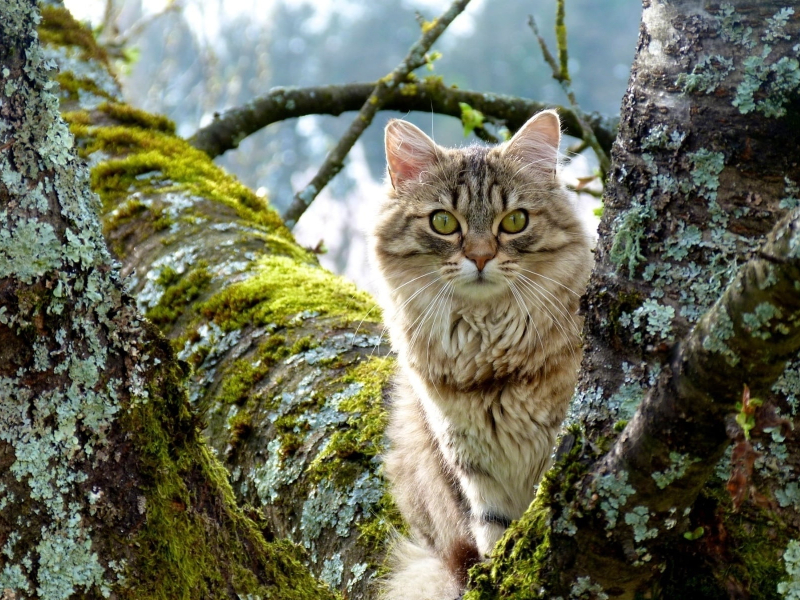
\includegraphics[width=0.5\textwidth]{image/cat.jpg}}
Các thông số của bức ảnh:
\begin{itemize}
    \item Kích thước: 800x600
    \item Số màu phân biệt trong ảnh (sử dụng numpy.unique): 158403
    \item Định dạng: JPEG
\end{itemize}

\subsection{Hình ảnh lúc sau (Số lần lặp = 100)}
Các phép đo, xử lý được thực hiện trên máy tính có cấu hình:
\begin{itemize}
    \item CPU: AMD Ryzen 7 5800H 8 nhân 16 luồng
    \item RAM: 32GB DDR4 3200MHz
    \item Hệ điều hành: Windows 10 Pro 64-bit
    \item Python 3.10.9 64-bit
\end{itemize}
Phép đo thời gian chạy sử dụng module time của Python và làm tròn đến 3 chữ số thập phân.
\subsubsection{k = 3, 5, 7}
k = 3: Thời gian chạy: 1.934s (random), 1.536s (in\_pixels) \\
k = 5: Thời gian chạy: 2.966s (random), 3.092s (in\_pixels)\\
k = 7: Thời gian chạy: 8.898s (random), 7.298s (in\_pixels)
\begin{figure}[h!]
  \begin{subfigure}{.5\textwidth}
    \centering
    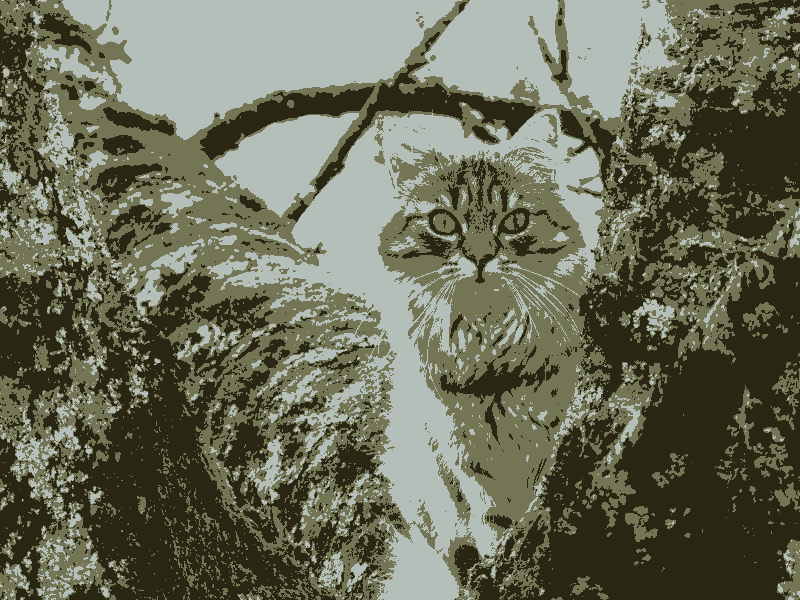
\includegraphics[width=.8\linewidth]{image/random_3.png}
    \caption{random}
    \label{fig:sfig1}
  \end{subfigure}%
  \begin{subfigure}{.5\textwidth}
    \centering
    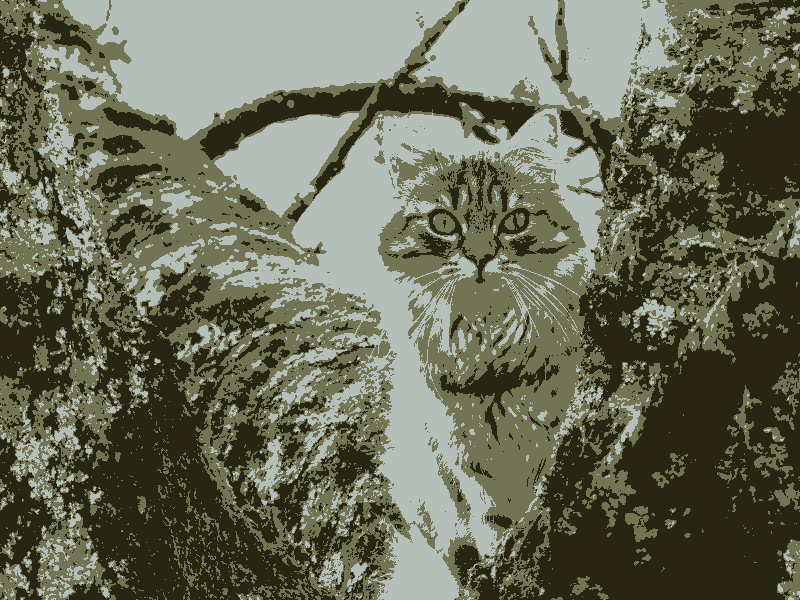
\includegraphics[width=.8\linewidth]{image/in_3.png}
    \caption{in\_pixels}
    \label{fig:sfig2}
  \end{subfigure}
  \caption{k = 3}
  \label{fig:fig}
\end{figure}

\begin{figure}[h!]
  \begin{subfigure}{.5\textwidth}
    \centering
    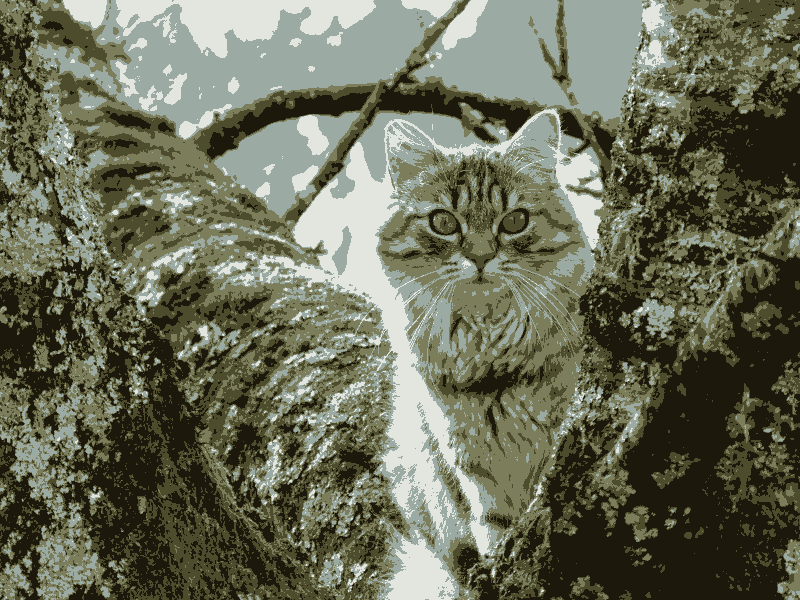
\includegraphics[width=.8\linewidth]{image/random_5.png}
    \caption{random}
    \label{fig:sfig3}
  \end{subfigure}%
  \begin{subfigure}{.5\textwidth}
    \centering
    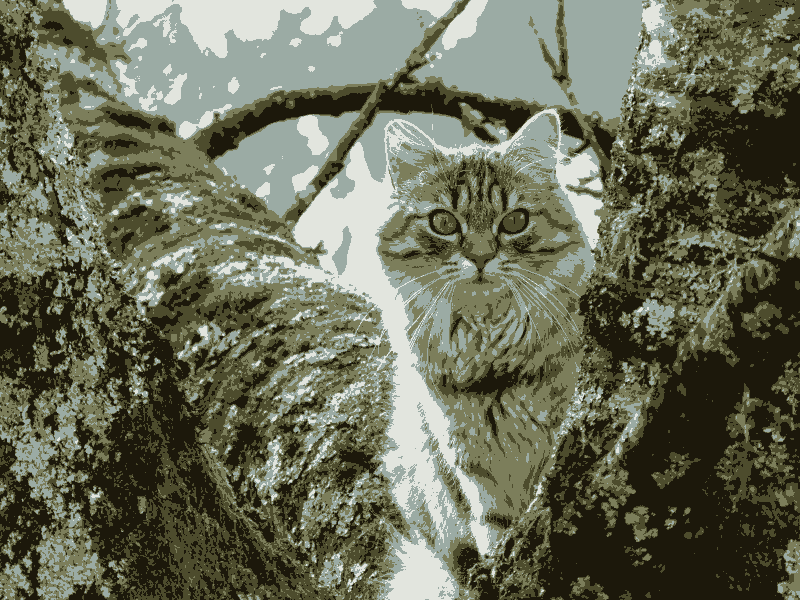
\includegraphics[width=.8\linewidth]{image/in_5.png}
    \caption{in\_pixels}
    \label{fig:sfig4}
  \end{subfigure}
  \caption{k = 5}
  \label{fig:fig1}
\end{figure}

\begin{figure}[h!]
  \begin{subfigure}{.5\textwidth}
    \centering
    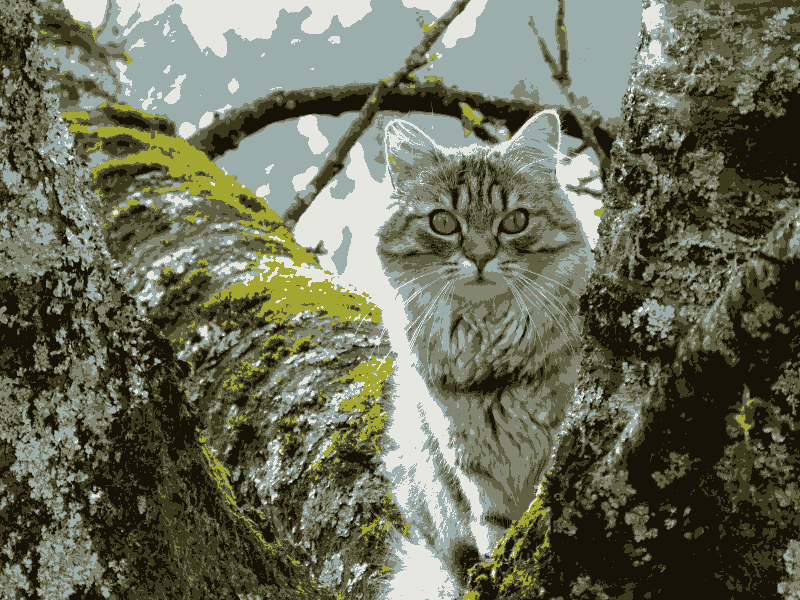
\includegraphics[width=.8\linewidth]{image/random_7.png}
    \caption{random}
    \label{fig:sfig5}
  \end{subfigure}%
  \begin{subfigure}{.5\textwidth}
    \centering
    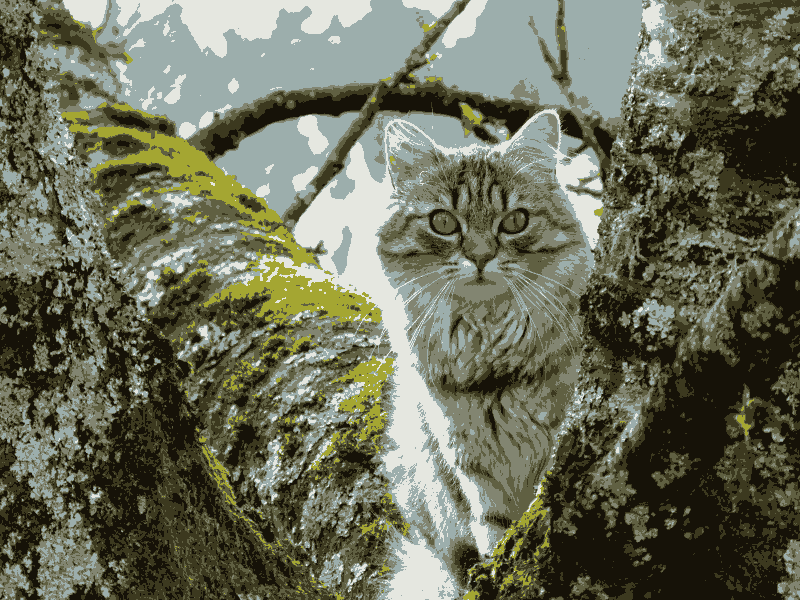
\includegraphics[width=.8\linewidth]{image/in_7.png}
    \caption{in\_pixels}
    \label{fig:sfig6}
  \end{subfigure}
  \caption{k = 7}
  \label{fig:fig2}
\end{figure}

\pagebreak
\subsubsection{k = 100, 256}
k = 100: Thời gian chạy: 139.685s (random), 143.472s (in\_pixels) \\ 
\begin{figure}[ht!]
  \begin{subfigure}{.5\textwidth}
    \centering
    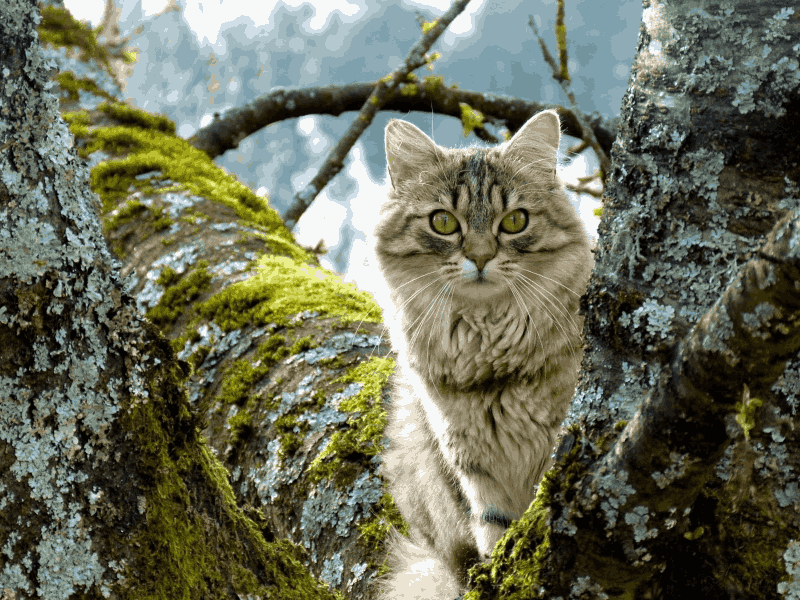
\includegraphics[width=.8\linewidth]{image/random_100.png}
    \caption{random}
    \label{fig:sfig7}
  \end{subfigure}%
  \begin{subfigure}{.5\textwidth}
    \centering
    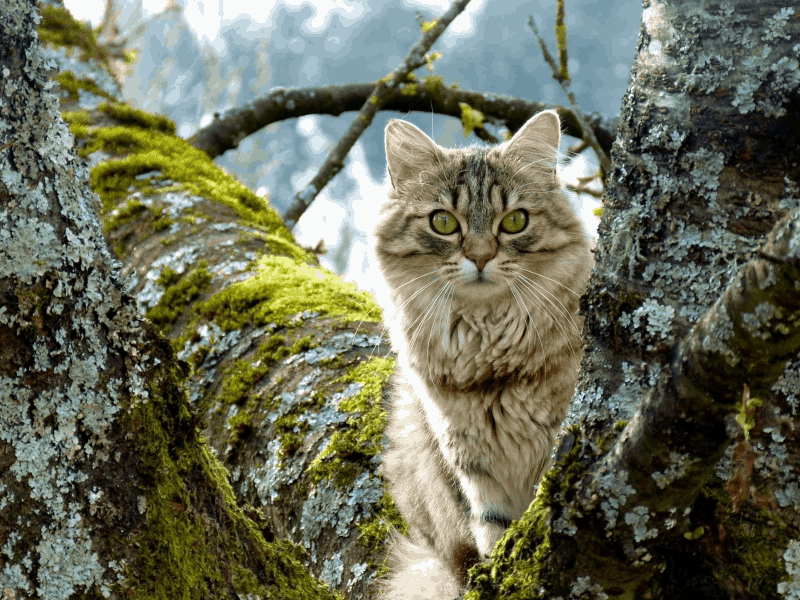
\includegraphics[width=.8\linewidth]{image/in_100.png}
    \caption{in\_pixels}
    \label{fig:sfig8}
  \end{subfigure}
  \caption{k = 100}
  \label{fig:fig3}
\end{figure}
k = 256: Thời gian chạy: 354.843s (random), 375.233s (in\_pixels)
\begin{figure}[ht!]
  \begin{subfigure}{.5\textwidth}
    \centering
    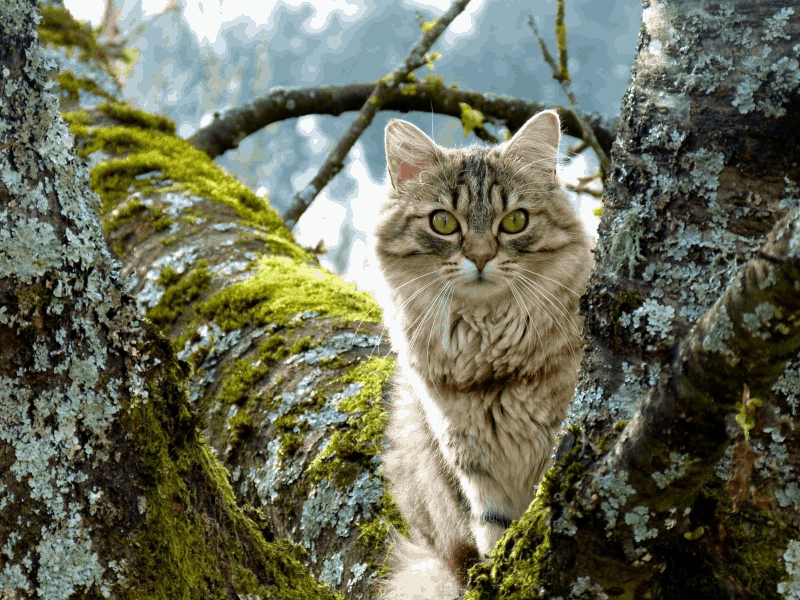
\includegraphics[width=.8\linewidth]{image/random_256.png}
    \caption{random}
    \label{fig:sfig9}
  \end{subfigure}%
  \begin{subfigure}{.5\textwidth}
    \centering
    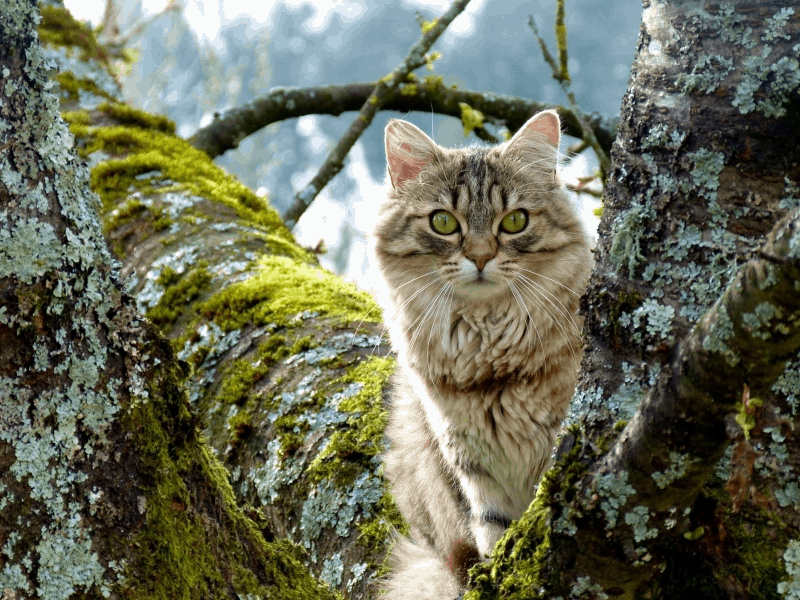
\includegraphics[width=.8\linewidth]{image/in_256.png}
    \caption{in\_pixels}
    \label{fig:sfig10}
  \end{subfigure}
  \caption{k = 256}
  \label{fig:fig4}
\end{figure}

\pagebreak
\newpage
\subsection{Nhận xét}
\subsubsection{Về ảnh đầu ra}
Trên lý thuyết, mắt con người có thể nhìn được hơn 10 triệu màu sắc khác nhau. Tuy nhiên, như kết quả thực nghiệm trên, khi k = 256, hình ảnh đã được phân cụm rất tốt, không có sự khác biệt đáng kể so với k = 100, trái lại thời gian còn tăng lên gấp đôi. \par

Quay trở lại 3 giá trị k nhỏ (3, 5, 7), ta thấy bức ảnh với k = 3 gần như trở thành bức ảnh đen trắng, không có sự phân đoạn rõ ràng. Khi k tiến lên bằng 5, một số chi tiết rêu xanh có thể nhìn rõ bằng mắt thường hơn. Và khi k = 7, ta có thể nhìn thấy chi tiết rêu xanh lá trên thân cây. \par

Với các giá trị k lớn (100, 256), do các màu sắc không có sự khác nhau đáng kể, nói nôm na là ''giống nhau'' nên sau khi xử lý bằng thuật toán K-Means, ta có thể nhìn các màu sắc gần như giống với bức ảnh gốc. Tại k = 100 ta có thể nhìn thấy các chi tiết rêu xanh lá không ''tươi'' bằng bức ảnh gốc, sự khác biệt này cải thiện rất nhiều khi tăng k = 256. \par

\begin{figure}[ht!]
  \begin{subfigure}{\textwidth}
    \centering
    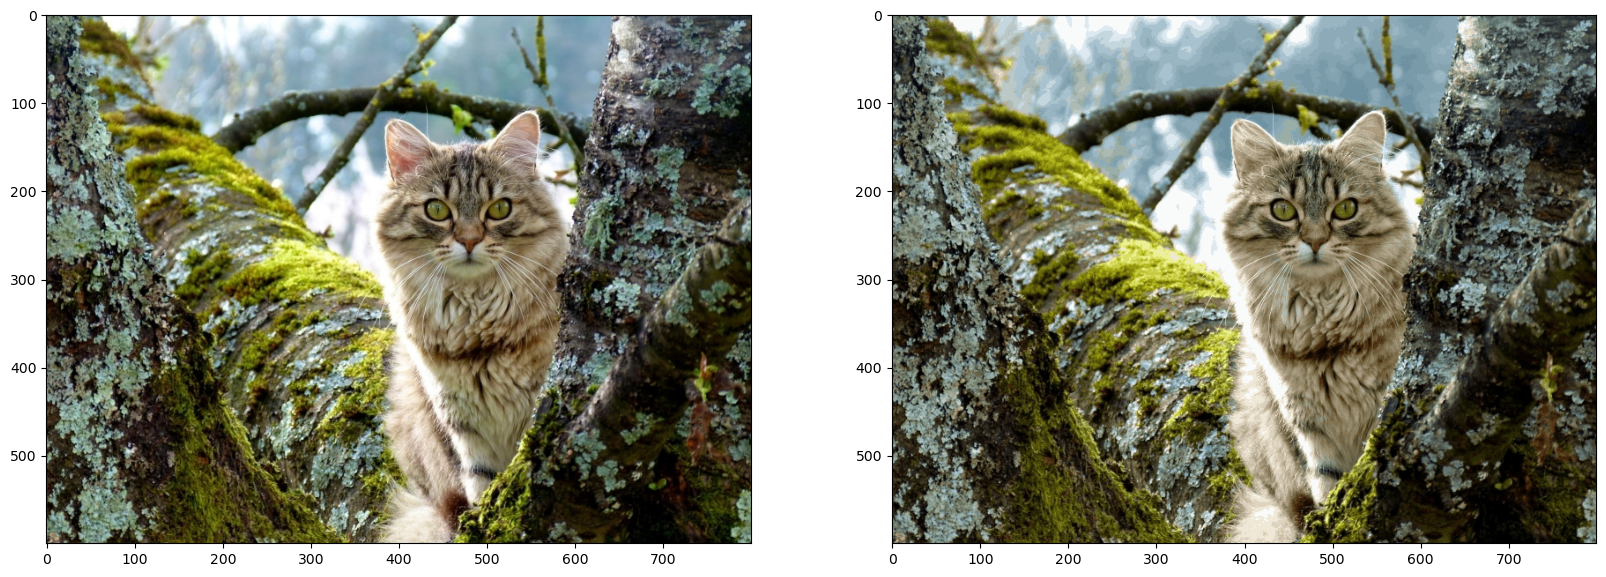
\includegraphics[width=\textwidth]{image/com_in_100.png}
    \caption{So sánh giữa bức ảnh gốc và bức ảnh được xử lý với k = 100 (in\_pixels)}
    \label{fig:sfig11}
  \end{subfigure}
  \begin{subfigure}{\textwidth}
    \centering
    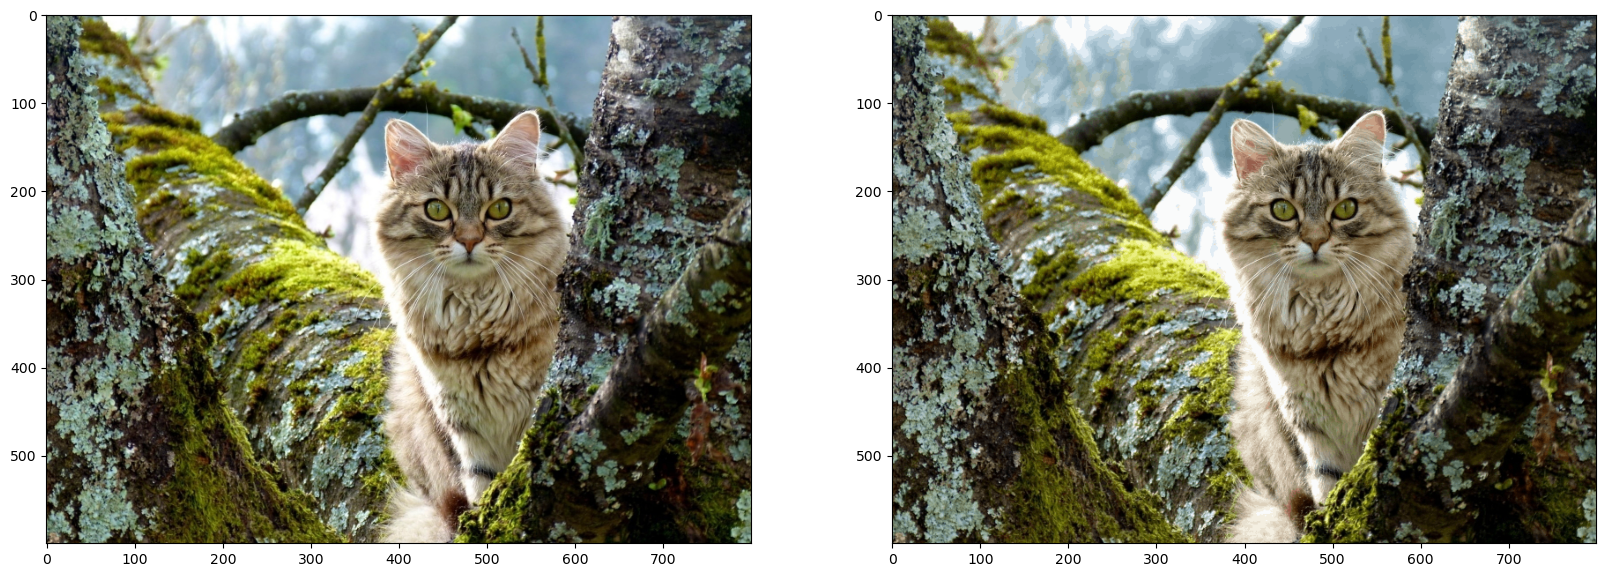
\includegraphics[width=\textwidth]{image/com_in_256.png}
    \caption{So sánh giữa bức ảnh gốc và bức ảnh được xử lý với k = 256 (in\_pixels)}
    \label{fig:sfig12}
  \end{subfigure}
  \label{fig:fig5}
\end{figure}

\newpage 
Bằng mẳt thường ta không thể phân biệt sự khác nhau giữa các bức ảnh xử lý bởi 2 kiểu khởi tạo centroid. Trong 3/5 trường hợp, thời gian chạy của kiểu khởi tạo in\_pixels lâu hơn đáng kể (khoảng 10\%) so với random. Điều này có thể giải thích bằng việc khi khởi tạo centroid theo kiểu in\_pixels, ta phải duyệt qua toàn bộ mảng unique\_img\_1d để lấy ra các điểm ảnh, trong khi đó, khi khởi tạo theo kiểu random, ta chỉ cần sinh ngẫu nhiên các giá trị trong khoảng [0, 255]. \par

\subsubsection{Về tài nguyên sử dụng}
Với các giá trị k nhỏ, hiệu năng CPU cần để tính toán là không đáng kể và kết quả trả về rất nhanh. Tuy nhiên trong trường hợp k = 256 với 100 vòng lặp, máy tính sử dụng khoảng 3.5GB RAM và 8.5\% CPU trong suốt quá trình chạy. \par

\centerline{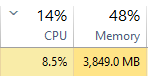
\includegraphics[width=0.2\textwidth]{image/performance.png}}
\newpage
\section{Tài liệu tham khảo}
\begin{itemize}
    \item \href{https://youtu.be/uLs-EYUpGAw?t=231}{How to Code K-Means in Python (No Sklearn)}
    \item \href{https://numpy.org/doc/stable/reference/generated/numpy.reshape.html}{numpy.reshape}
    \item \href{https://numpy.org/doc/stable/reference/random/generated/numpy.random.randint.html}{numpy.random.randint}
    \item \href{https://numpy.org/doc/stable/reference/random/generated/numpy.random.choice.html}{numpy.random.choice}
    \item \href{https://numpy.org/doc/stable/reference/generated/numpy.sum.html}{numpy.sum}
    \item \href{https://numpy.org/doc/stable/reference/generated/numpy.argmin.html}{numpy.argmin}
    \item \href{https://numpy.org/doc/stable/reference/generated/numpy.mean.html}{numpy.mean}
    \item \href{https://numpy.org/doc/stable/reference/generated/numpy.array_equal.html}{numpy.array\_equal}
    \item \href{https://matplotlib.org/stable/api/_as_gen/matplotlib.pyplot.figure.html}{matplotlib.pyplot.figure}
    \item \href{https://www.reddit.com/r/learnpython/comments/4g4dru/error_converting_images_to_pdf/}{Error converting images to pdf}
    \item \href{https://numpy.org/doc/stable/user/basics.broadcasting.html}{Broadcasting explained}
\end{itemize}

\end{document}